\documentclass{article}
\usepackage{graphicx} % Required for inserting images
\usepackage{layout}
\usepackage[margin=1in]{geometry}
\usepackage{setspace}

\title{Experimental Researches In Electromagnetism and Optics}
\author{Jack Norman}
\date{14 March 2025}
\doublespacing
\begin{document}

\maketitle

\section{Introduction}
In the selections of Faraday we read for class he concludes that magnetic and electrical phenomena are either identical aspects of the same force or deeply linked. In the penultimate Faraday reading of the semester he attempts to expand the dominion of these forces into light. He asserts that using a piece of lead glass encased in a solenoid one may bend light at will. Based on his writing it is unclear a) how one may quantify the amount of force applied to the light and b) whether there is any limit to the torsional angle exerted on the light. In order to answer these two questions I performed two experiments; the first to establish the relationship between current and magnetic force and the second to gather preliminary data on the torsion of polarized light. It was my hope that the results of the first experiment would give me a means of quantifying the force exerted on the light and in turn to provide me with an independent variable of the second experiment.

\section{Methods}
\subsection{Experiment I: Measuring Electromagnetic Force}
In Faraday's researches, before proving the mutual identity of static and voltaic electricity, he asserts that it is characteristic of voltaic electricity to register on a galvanometer whereas electric tension affects change in an electrometer and leaves a galvanometer unperturbed. From this I surmised that magnetism must be a function of current rather than tension, for one may observe extreme variation in electric tension without a change or production in magnetism. Despite these properties Faraday does not explicitly state the relationship between current and force. It is left to the reader to draw their own conclusion based on Faraday's assertion that the two phenomena are inseparable. If they are identical, it would follow that there would be a linear correlation of current with magnetism. In order to confirm that this was the case and not an alternative ratio I set out the following experiment.
\paragraph{}
I hypothesized that the quantity of magnetic force generated by the magnet would be in a linear proportion to the quantity of current passed through the coil. Because my goal was only to establish a proportion and not to produce a numerical account of the force exerted I chose to make use of Hooke's law. I first constructed an electromagnet and then affixed a ferrous nut to the end of a spring, gluing it in place. The other end of the spring was looped through an L shaped piece of copper sheet. After this the magnet was affixed to to the base of an upright yard stick with both leads connected to a DC power supply capable of generating 16 volts and 8 amps. I performed three trials of the following experiment with four settings of current for each which resulted in a total of twelve measurements.
\begin{enumerate}
    \item The power supply was adjusted to the amperage to be tested. I began with .5 amps and increased it by .5 amps with each test until it reached 2 amps. 
    \item I affixed the nut at the end of the spring to the upright end of the electromagnet.
    \item I placed the L shaped piece of copper against the yard stick and began to slowly move it up the yard stick counting off quarter inch intervals. 
    \item Once the nut sprang loose from the magnet I recorded the displacement on the chalkboard and repeated with the next level of current. (I began at .5 amps, went to 2 amps and then started a new trial.)
\end{enumerate}

\subsection{Experiment II: Measuring The Torsion of Light}
Faraday claims that he was able to bend light using a piece of leaded glass encased in an electrified solenoid but did not provide a proportion between current and deflection of the light nor even a degree measure of its deflection. He asserts that the reason for the light's refraction is solely based on its interaction with the magnetic field and the leaded glass only facilitates this interaction through a mysterious refractive property. Were this true I would expect the data to show a non linear trend whereby the rotation of the light was proportionally less with each addition of current. This is because in the use of a galvanometer the needle reaches a maximum deflection of 45 degrees and can scarcely be pushed further without a great addition of current. As we discussed in class this is because the direction of the needle is the resultant force vector of the gyre and the magnetic field lines of Earth. By this same reasoning if light were twisted solely by magnetism one would expect light itself to have some magnetic force which would resist the force of the magnet and as such would have a limit to its torsion. Likewise, the force exerted by the wire on the galvanometer is diminished in a greater than linear proportion as the distance from the galvanometer increases owing to the nature of magnetic dissipation. I contend that the rotation of the light owes rather to a change in the optical properties of the leaded glass precipitated by the magnetic field for two reasons: a) Faraday reports that other media seem to affect light with a "left hand rule" and b) that the glass contains a metallic component. \paragraph{}
If the phenomenon Faraday described was truly a function of magnetism alone one would imagine little change with an alteration of the medium save an diminished or increased intensity of torsion. I hypothesized that with each successive addition of current the torsion will be linearly increased as it depends on an alteration of the substance and not an alteration of the light directly. This is because I assumed that the bending of the light was owed to a deformation in the crystal lattice of the glass rather than a direct effect the magnetism had on the light. If this were the case, then as Taylor demonstrated, the deformation of the material at small displacements would exhibit curvature proportional with the inducing force. In order to gather such data I first set about modifying a polarized lens to be adjustable by degrees. First I measured the circumference of a polarized lens. Then a paper strip was cut of the same length and a millimeter ruler was used to evenly divide it into 18 sections, each corresponding to 20 degrees. After this the intervals were further subdivided to provide 180 with each corresponding to two degrees. 

This lens was then placed on a mount closest to a white sheet of paper taped to the wall. Aside from the measuring tape affixed to the lens the remainder of the setup was identical to the "Faraday Effect" practicum. With this setup in place the following procedure was executed.
\begin{enumerate}
    \item The frontal lens was adjusted to darken the laser on the wall to its minimum brightness. 
    \item The DC power supply was set to provide the correct amount of current. 
    \item With the laser once again visible (on account of the supposed torsion), the lens was rotated until the light once more was diminished. After this, the degree measurement of the turn was recorded. 
    \item The power supply was cycled off and the process was once again repeated. 
\end{enumerate}
In the above experiment current was tested from one to eight amperes with steps of one ampere for each measurement. Only one trial of this experiment was completed owing to a lack of precision. It is included in this write up only to provide a blueprint for future investigation and to provide a foil for the discussion of electromagnetic force. 
\newpage
\section[t]{Results}

\begin{figure}[h]
\centering\textbf{Measuring Electromagnetic Force}
    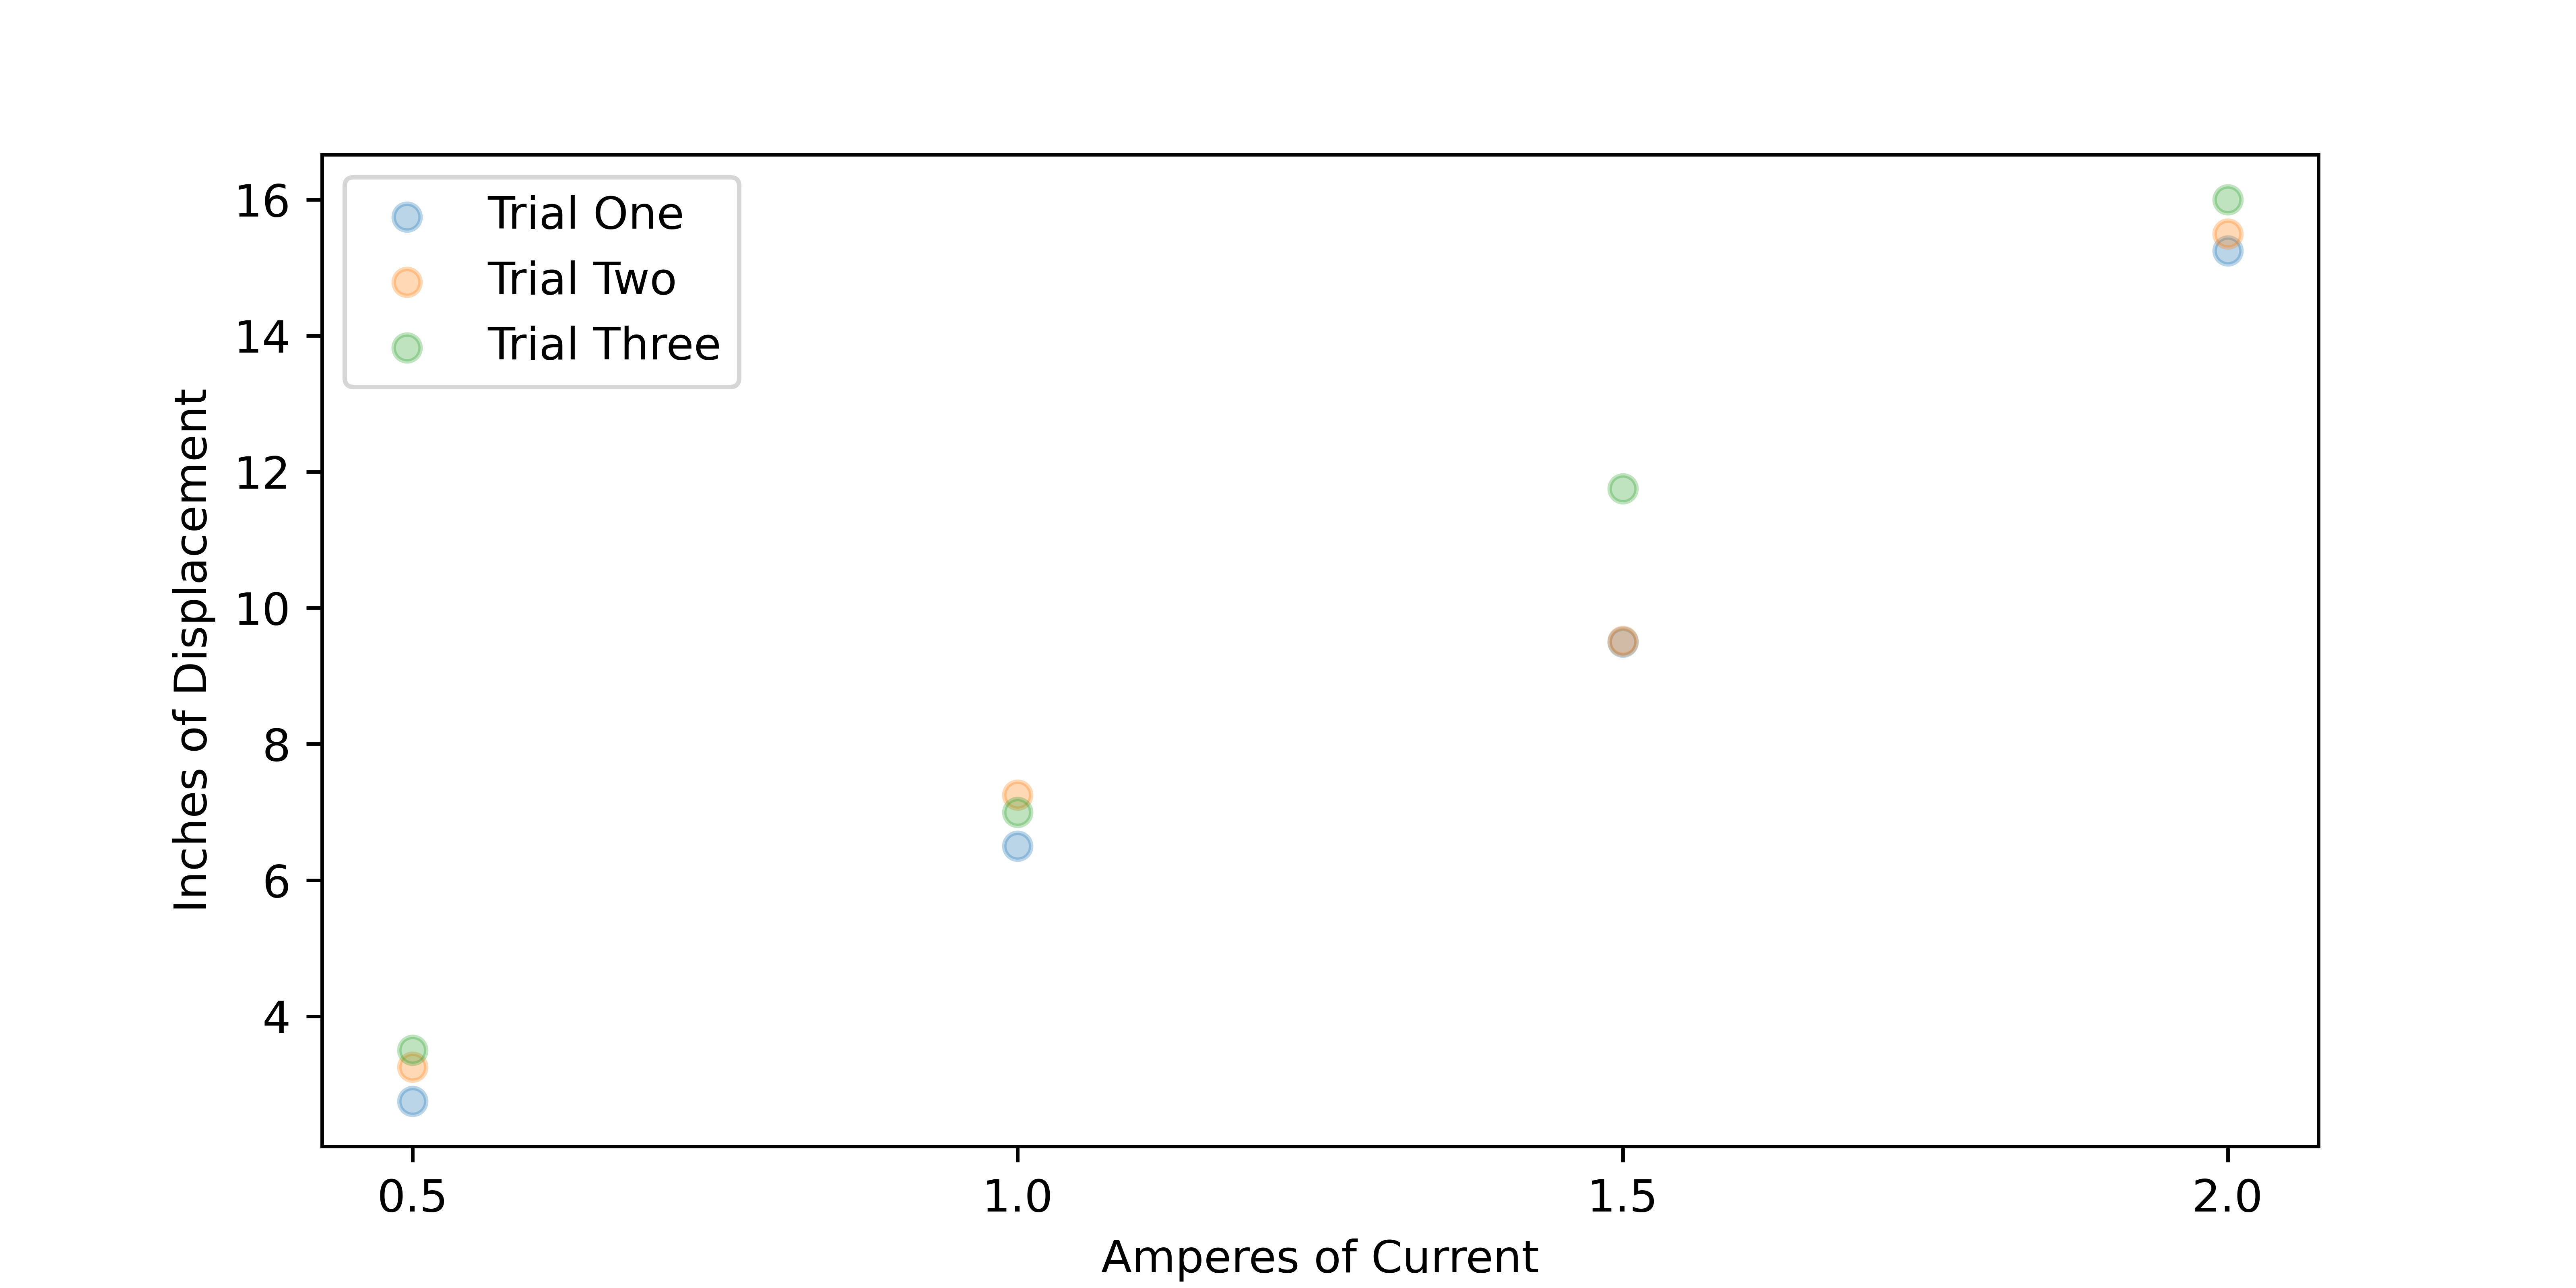
\includegraphics[width=.75\linewidth]{amps_vs_dispv0.png}
\end{figure}


\begin{figure}[h]
    \centering\textbf{Measuring Photonic Torsion}
    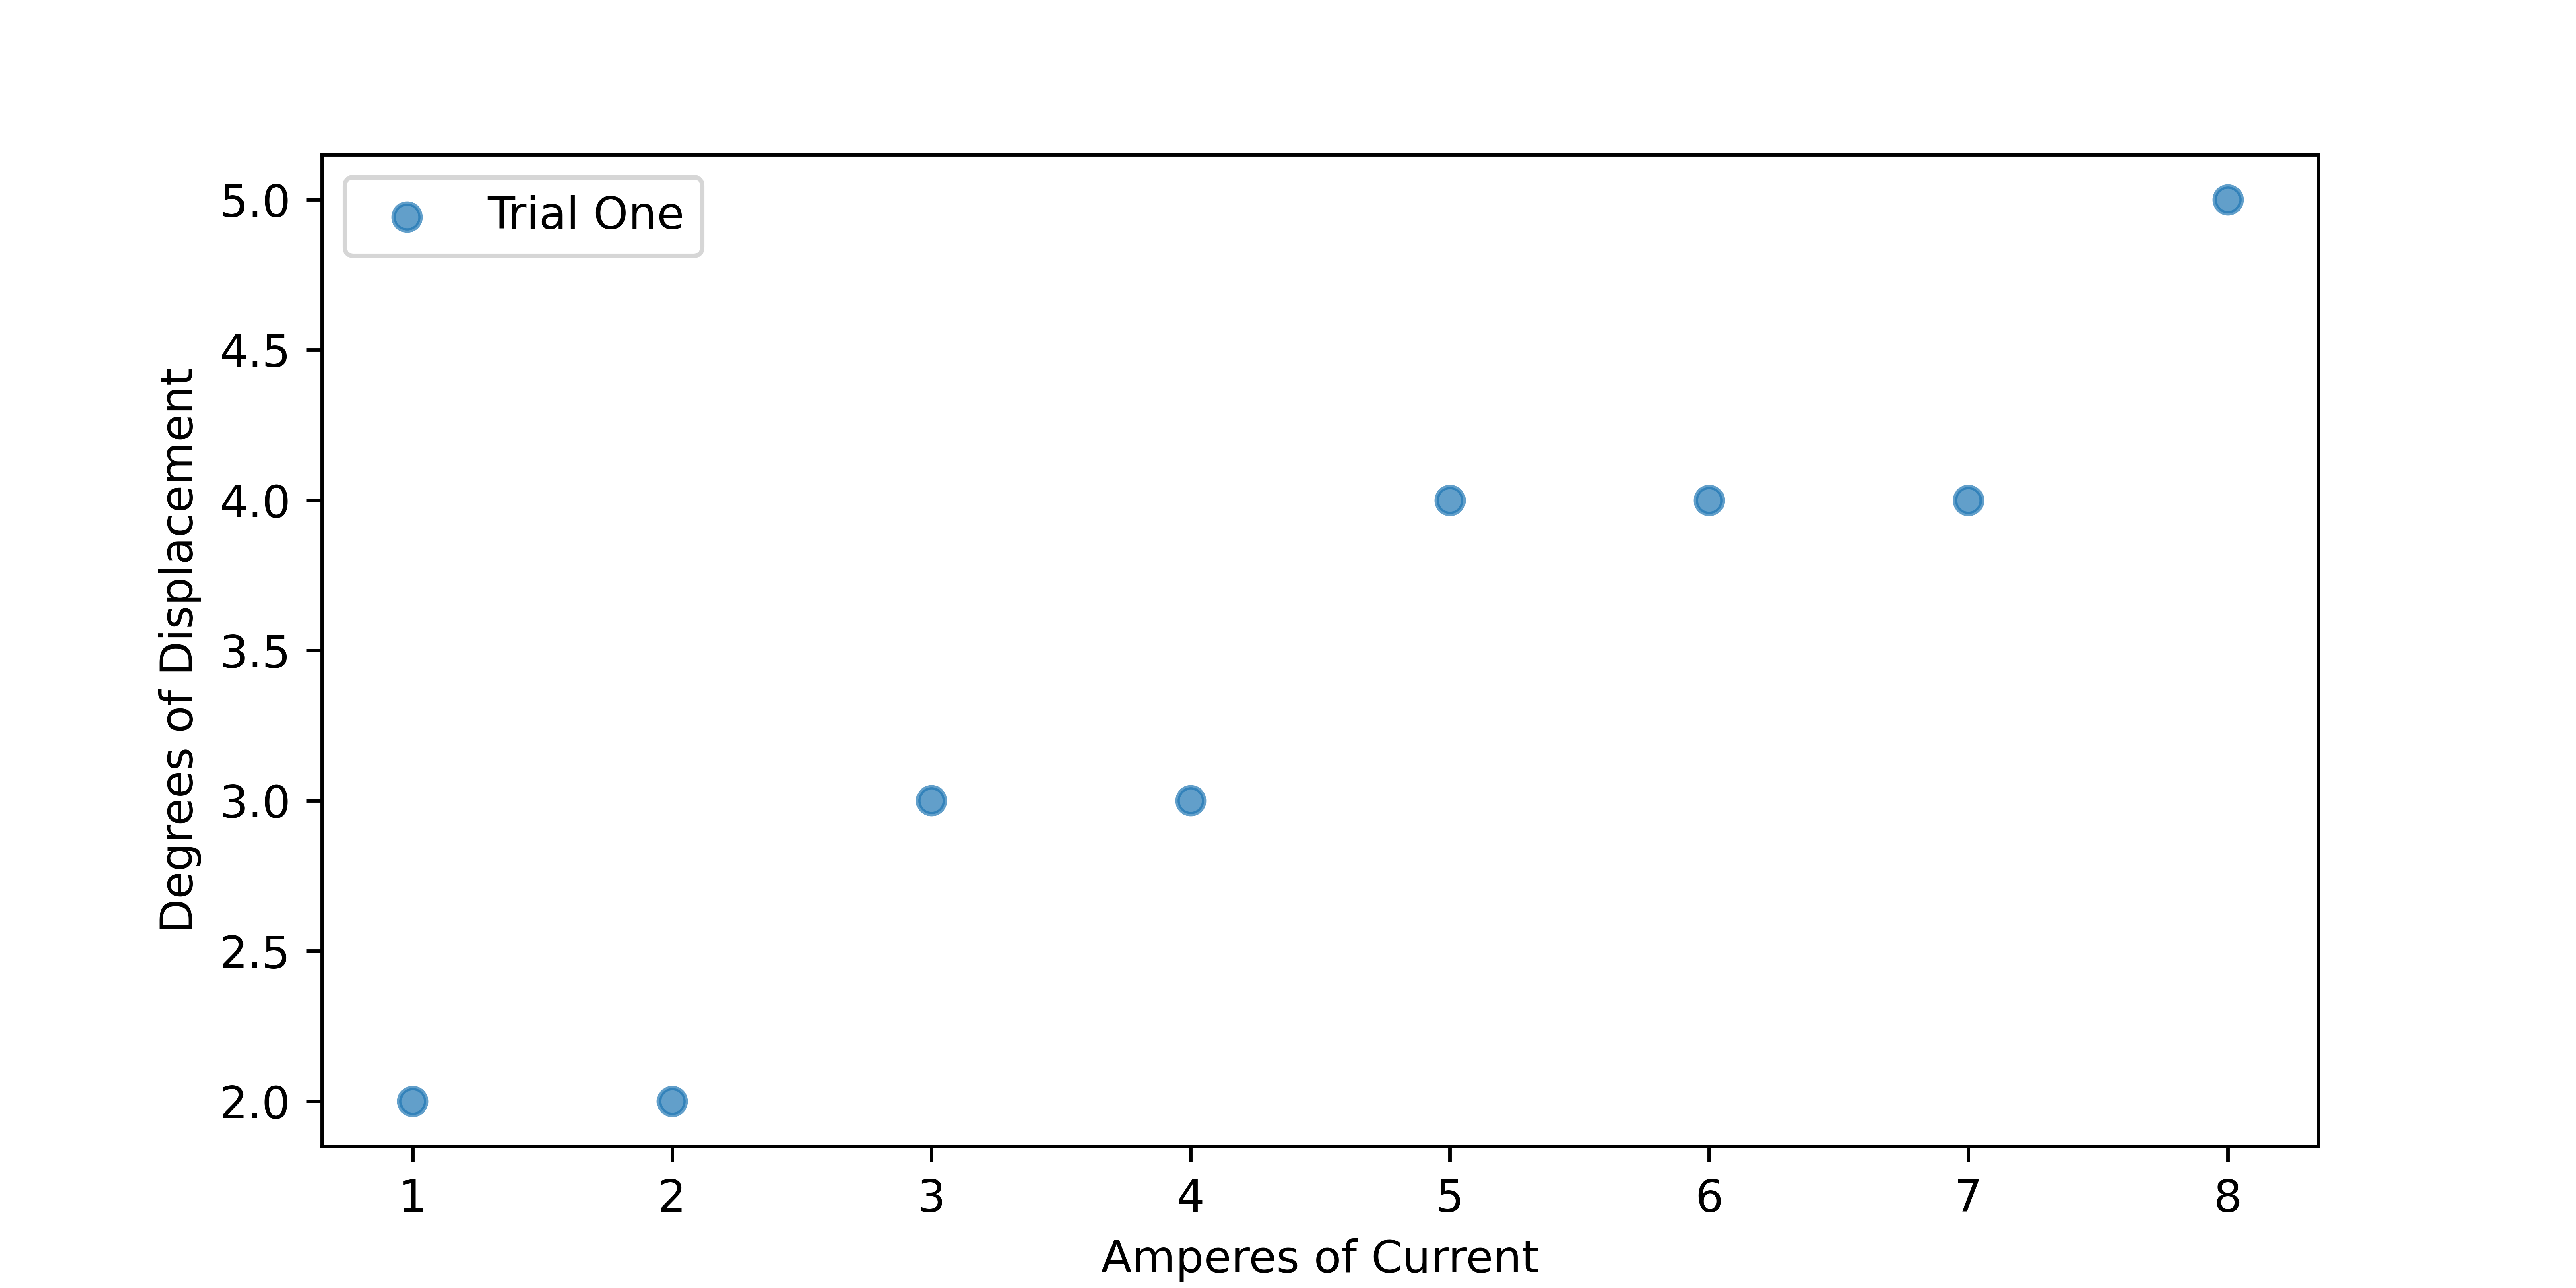
\includegraphics[width=0.75\linewidth]{amps_vs_degrees.png}

\end{figure}

\newpage
\section{Discussion}
The data provided by the first experiment support the hypothesis that the amount of magnetic force at a set distance scales linearly with the addition of current as measured in amperes. The data form tight clusters with a linear trend upwards as a function of amperage. More trials will be necessary to assert with confidence that there is a causal rather than merely correlative relationship between the two, but if there is a causal relationship then I assert that the data's departure from it owes to two sources. The first source is a gradual destruction of the spring's elastic power owing to high displacements. Likewise, the measurements were taken by eye and with quarter inch precision so if the nut sprang free in between I was powerless to find a more precise number than my last count without a reliance on invention. The first source of error is supported by the positions of each of the data points relative to the others at the same current with the third trial as the highest in three out of four, the second second in three out of four, and the first lowest in all. These results are consistent with the idea that as the experiment progressed the spring weakened and in turn allowed a greater displacement before breaking the nut free.\paragraph{} While evaluating the experiment it occurred to me that I ran the risk of circularity with my experiment design; if, like a galvanometer, amperage measures the amount of magnetism produced by a wire endowed with electricity, then it comes as little surprise that it should have a relationship with magnetism. Even if this were true, I did not have a prior understanding of the relationship between a number in amperes and the amount of force generated by a magnet created by it. In fact, it is in no way obvious nor even plausible that the deflection of a galvanometer is linearly related to the amount of current in a wire. This is evidenced both by its maximum deflection of 45 degrees and the changing angle between the gyre and the position of the needle. On the other hand, it is now clear that an ampere \textit{does} represent a linear increase in magnetic force. While these findings do little to inform me of the true nature of current and electricity, they provide a valuable tool for the investigation of the torsion of light. \paragraph{}
I hold the results obtained from the photonic torsion experiment are under such extreme suspicion that I will refrain from any speculation concerning their cause or meaning. As such, the hypothesis that the bending of light is dependent on the medium in conjunction with magnetism and not the medium alone is undecidable. In future researches I will devise a more sensitive and objective means of evaluating the brightness of the light on the wall and will manufacture a vernier dial to obtain a greater degree of precision in the rotation of the lens. The points of failure in my experiment design were twofold and could be remedied with sufficient preparation. The first was a woefully imprecise measuring apparatus for the minute shifts characteristic of the light. The second source of error was the subjectivity regarding the brightness of the laser. In order to address this problem I could employ a photo detector shielded from other light in the room which would ensure an accurate reading and would also indicate whether the light could always be darkened to the same degree.  
\section{Conclusion}
This paper dealt with two lines of inquiry: a) the relationship between current and the magnetic force generated by a solenoid and b) the relationship between magnetic force and the torsion of light. Regarding the first problem it was hypothesized that owing to supposed identity of magnetism with electricity there should be a linear relationship between current and magnetism. Following an experiment deploying Hooke's law, the hypothesis was supported and I conclude that there is at least a strong correlation between the quantity of electric current and the force of magnetism. During this same experiment I noticed that placing the ferrous nut at a point in space above the magnet and achieving static equilibrium was a fool's errand. It seemed that the magnetic force was all but absent (it pulled the nut no more than a tenth of an inch) then suddenly would seize its quarry and hold it fast. I suspected that the strength of the magnet would decrease according to a similar rule as gravity but after observing this phenomenon I am skeptical that such a thing is true under the conditions I was working. Viz. under small displacements the magnet's power seemed to vary more rapidly according to displacement than the inverse square law would suggest. Regardless of the relationship, I was satisfied having obtained the proportion between current and magnetism. Brandishing this conclusion in hand I set out to evaluate the degree of torsion of polarized light under the influence of a solenoid using the same setup as was used in class but with the addition of degree measurement. I hypothesized that once more there would be a linear relationship between the current exerted and the degree of torsion exhibited and that this relationship would increase linearly until it stopped abruptly. Because of the crudeness of my measuring devices, fabricated by none other than I, I was forced to classify my hypothesis as undecidable. 

\end{document}
